\chapter{多版本缓冲事务技术及文件系统效能优化}
\label{chap:vct}

\section{文件系统及效能优化}

\subsection{现有文件系统设计和页缓存}

\subsection{文件系统对应用效能的影响}

\subsection{数据一致性和滞后性}

\section{以内存为中心的文件系统}

\subsection{设计原则}

\subsection{系统架构}

\begin{figure}
  \centering
  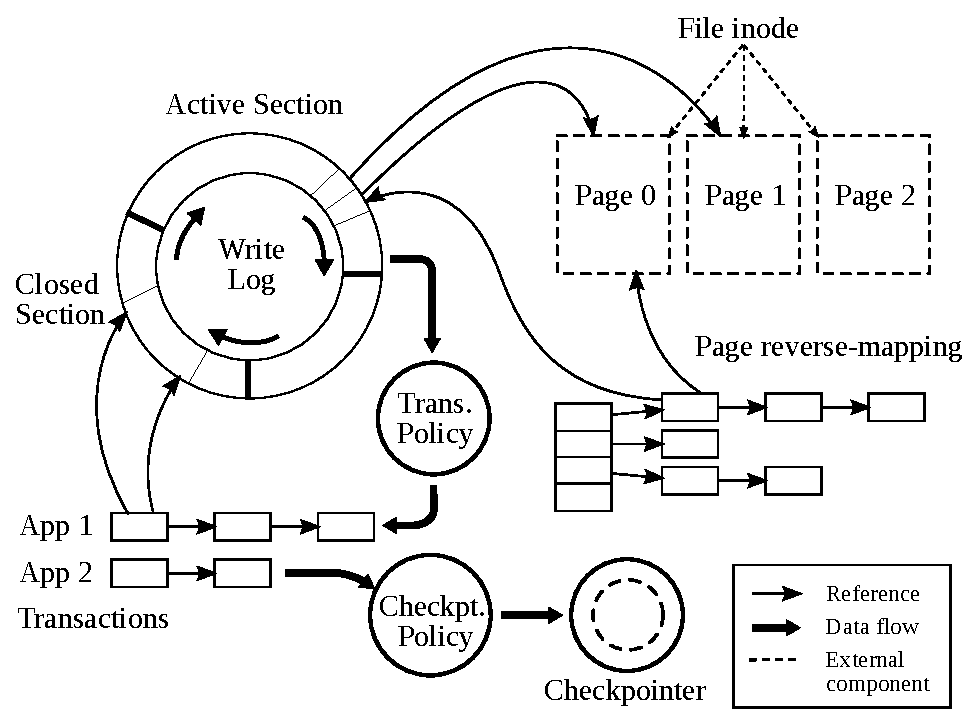
\includegraphics[width=0.8\columnwidth]{arch}
  \caption{MobiFS系统架构图}
  \label{fig:arch}
\end{figure}

MobiFS主要由五个模块构成:(1)页缓存,负责在内存中存储文件数据;(2)写日志,负责维护写操作的历史,由按序排列的许多记录项构成;(3)事务,写日志中的若干记录项归并为一组,它们的一致性不受覆写和重排序等优化的影响;(4)检查点生成器(checkpointer),负责调用底层闪存存储组件以原子性方式完成事务的持久化;(5)策略引擎,负责依据优化算法划分事务的边界,监听用户交互行为,并决定生成检查点的事务和时机。图~\ref{fig:arch} 描绘了MobiFS的系统架构。

MobiFS的设计充分考虑了与现有操作系统(Linux)的兼容和组件重用。它与操作系统共享现有的页缓存结构。对于页缓存的每个写操作,都会记入写日志,通常体现为在当前事务中(写日志的末尾)追加一个记录项,除非当前事务已经包含目标页地址的记录项。为此,我们需要维护一组从页地址到写日志项的逆向映射,以判断目标页地址是否已经存在于事务中。基于写日志和逆向映射,MobiFS建立起原子性事务机制。每个事务定义了可以进行覆写和重排序等优化的一个特定范围。最终,策略引擎指导检查点生成器保存事务到闪存,同时不影响用户交互。策略引擎根据每个手机应用甚至是用户的行为及其统计指标,做出动态的智能的判断。

在一个典型的配置中,不同手机应用会拥有自己独立的写日志和事务,但它们共享逆向映射、策略引擎和检查点生成器等组件。

\section{多版本缓冲事务技术}

\subsection{写日志}

写日志是应用所有写操作按时间排列的历史记录。写日志包含两个段:活跃段(active section)处在写日志的末尾,新的记录项会被插入活跃段;闭合段(closed section)则包含准备生成检查点的记录项。 
 
在Android平台上,一份写日志的范围涵盖一个手机应用访问的所有目录。手机应用可能使用数据库SQLite保存数据,而SQLite是一个嵌入式数据库,它与每个应用捆绑的相关文件也需要托管给MobiFS,包含在应用的写日志范围内。
 
我们之所以能够面向特定应用进行写优化,一个重要原因在于手机应用的数据路径是静态的和相互隔离的,从而避免了应用间的一致性问题。当然,的确存在多个应用共享文件数据的情况,例如文件浏览器和相册应用可能同时管理照片存放的目录。这种情况下,相关应用需要在程序逻辑层面进行处理。即便不使用MobiFS,在现有Android的文件系统上,应用同样需要处理这类情况(例如,用户通过文件浏览器手动删除了相册中原本可见的照片)。 

\subsection{事务和版本}

在写日志中,可能同时存在逻辑上同一个缓冲页的多个物理版本。多版本缓冲事务用来管理这种关系。一个多版本缓冲事务在其生命周期内经历三个状态:(1)当处于打开状态时,一个事务接收新的记录项,而这些记录项构成写日志中的活跃段。(2)当进入闭合状态时,该事务的所有记录项不再可以更改,转入写日志的闭合段。从打开状态到闭合状态的转换是单向的,不可逆的。(3)当进入提交状态时,该事务所有记录项对应的物理缓存页被检查点生成器原子性地刷出到闪存。成功提交之后,该事务及其记录项即从写日志中消除。 
 
覆写和重排序等优化手段只允许用于单个多版本缓冲事务内部。由于检查点生成器可保证一个事务整体的持久化和原子性,这些优化不会导致闪存数据的任何不一致状态。 
 
当一个写操作到达时,MobiFS需要处理三种情况:(1)如果要写入的目标页不存在于逆向映射中,那么意味着写操作将进入一个未被写日志涵盖的页。MobiFS会在写日志中追加一个记录项,建立到缓存页的映射,并建立逆向映射。(2)如果逆向映射已经存在且指向一个写日志闭合段中的记录项,那么意味着写操作想要写入一个被保护的只读的事务。为此MobiFS对目标页执行写时拷贝(copy-on-write),并为新的页副本添加写日志记录项及映射/逆向映射。(3)如果逆向映射存在且指向一个写日志活跃段中的记录项(即打开的事务),那么意味着目标页不在被保护的闭合事务中,写操作可以直接更改目标页。

\subsection{故障恢复}

\subsection{检查点生成}

\section{效能优化策略和算法}

\subsection{概述}

\subsection{事务划分算法}

\subsection{行为间隔预测}

\subsection{事务调度}

\section{系统实现和效能评测}

\subsection{系统实现}

\subsection{评测方法}

\subsection{内存占用评测}

\subsection{应用和用户感知评测}

\subsection{应用响应度评测}

\subsection{能耗评测}

\section{本章小结}

